%%%%%%%%%%%%%%%%%%%%%%%%%%%%%%%%%%%%%%%%%
% The Commander X16 User's Manual
%
% Authors:
% Jestin Stoffel (jestin.stoffel@gmail.com)
%
% License:
% CC BY-NC-SA 4.0 (https://creativecommons.org/licenses/by-nc-sa/4.0/)
%
% Compiling this template:
% This template uses biber for its bibliography and makeindex for its index.
% When you first open the template, compile it from the command line with the 
% commands below to make sure your LaTeX distribution is configured correctly:
%
% 1) pdflatex main
% 2) makeindex main.idx -s indexstyle.ist
% 3) biber main
% 4) pdflatex main x 2
%
% After this, when you wish to update the bibliography/index use the appropriate
% command above and make sure to compile with pdflatex several times 
% afterwards to propagate your changes to the document.
%
%%%%%%%%%%%%%%%%%%%%%%%%%%%%%%%%%%%%%%%%%

%----------------------------------------------------------------------------------------
%	PACKAGES AND OTHER DOCUMENT CONFIGURATIONS
%----------------------------------------------------------------------------------------

\documentclass[
	11pt, % Default font size, select one of 10pt, 11pt or 12pt
	fleqn, % Left align equations
	letterpaper, % Paper size, use either 'a4paper' for A4 size or 'letterpaper' for US letter size
	%oneside, % Uncomment for oneside mode, this doesn't start new chapters and parts on odd pages (adding an empty page if required), this mode is more suitable if the book is to be read on a screen instead of printed
]{CommodoreBlueBook}

% Book information for PDF metadata, remove/comment this block if not required 
\hypersetup{
	pdftitle={Title}, % Title field
	pdfauthor={Author}, % Author field
	pdfsubject={Subject}, % Subject field
	pdfkeywords={Keyword1, Keyword2, ...}, % Keywords
	pdfcreator={LaTeX}, % Content creator field
}

\setlength\parindent{0pt}

\addbibresource{sample.bib} % Bibliography file

\definecolor{blue}{rgb}{0.0,0.0,0.8}
\definecolor{gray}{rgb}{0.73, 0.73, 0.73}

%----------------------------------------------------------------------------------------

\begin{document}

%----------------------------------------------------------------------------------------
%	COVER PAGE
%----------------------------------------------------------------------------------------

\coverpage % Output the title page
	{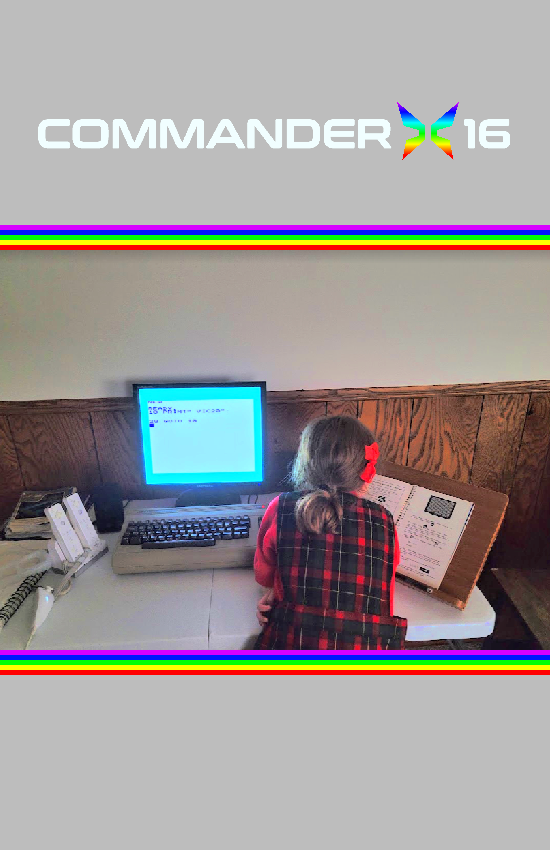
\includegraphics[width=\paperwidth]{cover.png}} % Code to output the background image, which should be the same dimensions as the paper to fill the page entirely; leave empty for no background image
	{ % Title(s) and author(s)
		\centering\rmfamily % Font styling
		{\Huge\bfseries Retro Computing on the\par} % Top
	}
	{
		\centering\rmfamily % Font styling
		{\huge\bfseries a friendly computer guide\par} % Bottom
	}

%----------------------------------------------------------------------------------------
%	COPYRIGHT PAGE
%----------------------------------------------------------------------------------------

\thispagestyle{empty} % Suppress headers and footers on this page

~\vfill % Push the text down to the bottom of the page

% \noindent \textsc{Published by Publisher}\\ % Publisher

\noindent \textsc{\href{https://www.commanderx16.com}{commanderx16.com}}\\ % URL

\noindent \textit{1st Edition}\\ % Printing/edition date

\noindent Copyright \copyright\ 2022 Jestin Stoffel\\ % Copyright notice

\noindent Licensed under the Creative Commons Attribution-NonCommercial 4.0
License (the ``License''). You may not use this file except in compliance with
the License. You may obtain a copy of the License at
\url{https://creativecommons.org/licenses/by-nc-sa/4.0}. Unless required by
applicable law or agreed to in writing, software distributed under the License
is distributed on an \textsc{``as is'' basis, without warranties or conditions
of any kind}, either express or implied. See the License for the specific
language governing permissions and limitations under the License.\\ % License information, replace this with your own license (if any)

\cleardoublepage % Start the following content on a new page

% start roman page numbering
\pagenumbering{Roman}

%----------------------------------------------------------------------------------------
%	TITLE PAGE
%----------------------------------------------------------------------------------------
\pagecolor{blue}

\afterpage{
	\thispagestyle{part} % use part header/footer style
	\newgeometry{
		top=1.5in, % Top margin
		bottom=-0.25in, % Bottom margin
		right=0.75in, % Right margin
		}
	\begin{flushright}
		{
			\huge\sffamily\bfseries\color{white}
			RETRO\\ COMPUTING\\ ON THE\\
			\vspace{8pt}
			{
				\contourlength{2pt}
				\contournumber{20}
				\fontsize{36pt}{36pt}\selectfont Commander
				\contour{white}{\textcolor{blue} {X16}}
			}
		}
		\huge\sffamily\color{white} A friendly computer guide
	\end{flushright}
	\restoregeometry
	\clearpage
}

\clearpage

\nopagecolor % Change page color back

%----------------------------------------------------------------------------------------
%	PREFACE
%----------------------------------------------------------------------------------------

%----------------------------------------------------------------------------------------
%	PREFACE PAGE
%----------------------------------------------------------------------------------------

\section*{PREFACE}
\addcontentsline{toc}{chapter}{\protect\numberline{}PREFACE}

\par You are about to meet a computer that feels out of place for its time.  It
is slower, larger, and more expensive than most computers of its era.  In many
ways, it is a technological anachronism designed for a niche market of
hobbyists and enthusiasts.  But that's not all.

\medskip
\par The Commander X16 reaches into the past and brings back many things that
were lost.  It is a computer that recaptures the "soul" of the early days of
home computing.  Together with this manual, anyone should be able to sit down
and begin to explore computing with all the modern layers of abstraction
stripped away.  No prior knowledge of computing or even typing should be
required in order to start your journey into the world of computers!

\medskip
\par This manual should be readable by experts and novices alike.  Even children as
young as 6 or 7 should be able to follow along with the step-by-step examples.
There is no reason you need to read this manual in order.  After reading
Chapter 1 (Getting Started) you can go directly to a chapter that interests you
and start reading.  The first page of each chapter contains a small sample
program to type in.  Type it exactly for a demonstration of what you will learn
in that chapter.  The rest of the chapter will explain the details as you read,
and contain more sample programs to try out.

% \medskip
% \par The Commander X16 was created with the intention that you can simply turn it on
% and start learning, doing, and creating.  The friendly blue screen and colorful
% butterfly logo invite you to start typing BASIC commands and programs.  The
% built-in SD card reader allows you to save your work as well as load the
% programs and art that others create, all without needing to troubleshoot
% expensive antique disk drives and data sets...although it supports those too!

\medskip
\par Computers have become an important part of our everyday lives, and yet most
people never delve past the surface of the user interfaces presented to them.
Children are given touch screen devices before they can even talk, and adults
go through their entire lives without learning about the magic that happens
behind their screens.  The Commander X16 reverses this trend by putting the
user back in control of a computer that they can fully understand.

\medskip
\par The Commander X16 is the perfect computer for this day and age!


%----------------------------------------------------------------------------------------
%	TABLE OF CONTENTS
%----------------------------------------------------------------------------------------

\pagestyle{empty} % Disable headers and footers for the following pages

\setcounter{tocdepth}{0}
\tableofcontents % Output the table of contents

% \listoffigures % Output the list of figures, comment or remove this command if not required
% 
% \listoftables % Output the list of tables, comment or remove this command if not required

\pagestyle{fancy} % Enable default headers and footers again

\clearpage % Start the following content on a new page

%----------------------------------------------------------------------------------------
%	SETUP
%----------------------------------------------------------------------------------------

%----------------------------------------------------------------------------------------
%	SETUP PAGE
%----------------------------------------------------------------------------------------

\section*{SETUP}
\addcontentsline{toc}{section}{\protect\numberline{}SETUP}

Autem eos placeat est in iure. Qui tempora ut ut qui dolores unde. Nesciunt
omnis cum iusto laboriosam ut. Amet similique omnis sit maxime laudantium.
Nobis delectus ut corrupti et excepturi. Aut amet error cumque eaque explicabo
quo unde. Minus consectetur error atque ut. Alias ut repudiandae eum eum.
Quaerat rerum facilis suscipit dolores qui consequatur aut perferendis. Et
alias est autem fugit enim nobis qui illo. Error nesciunt et adipisci ex
nostrum. Laudantium sit et ut est voluptatum dolor. Ea vitae soluta consectetur
vel culpa reiciendis. Ad est officiis ut consectetur sint voluptatem aut dolor.
Tempora consequuntur suscipit asperiores exercitationem. Harum officia nisi
omnis ut iste rerum. Consequatur tempora maxime ipsa velit sit. Consequatur
ipsum necessitatibus autem ut saepe eum quod ea. Omnis qui non et minima
perferendis sunt repudiandae. Voluptas minima earum est libero inventore
corporis est sint. Occaecati odio distinctio est. Ab quidem asperiores deleniti
soluta debitis exercitationem veniam. Ut sit quo accusantium velit quam
voluptatum quia quia. Non sed non consequatur corrupti sed libero. Vitae
dolores id distinctio enim magni sed omnis.

Voluptates ipsa animi et a iusto. Qui doloribus ducimus voluptas sunt quidem
similique animi blanditiis. Cupiditate dolorum quia illo. Totam sit consequatur
quos. Ipsa dolorum dolor dolores ad deserunt eum debitis. Id quae porro
eligendi tempora magni qui odit. Recusandae et placeat officia blanditiis
perspiciatis quaerat. At saepe perspiciatis explicabo. Non sit quam
exercitationem sequi commodi tempore et quasi. Tempora distinctio et voluptatum
reiciendis qui minus deleniti. Quidem officiis eveniet debitis voluptas sint
provident numquam architecto. Eligendi quibusdam rerum debitis possimus et
ratione enim quasi. Placeat minus beatae sed aut est. Itaque quisquam eum
adipisci enim rerum qui. Dolor at veniam est molestiae. Sed velit sunt est
consequatur suscipit. Quisquam et ipsum qui est et accusantium porro omnis.
Asperiores enim eos eos. Unde officiis quo est ex expedita odit. Vel maiores
animi non dolor molestiae quia rerum aut. Vel tempore non doloremque sint
nesciunt. Ipsa voluptas qui repellat id earum temporibus ut soluta. Pariatur
esse beatae autem et consequatur repellendus cum dolores. A aliquam porro
voluptatem repellat dolorem. Doloribus voluptas aspernatur in veniam est iusto.

Eveniet dolorum maiores vitae. Rerum culpa et consequatur. Cumque tenetur
dolorem autem voluptatum. Omnis aut nihil odio ipsam et. Fugiat fuga molestias
earum ut neque odit. Cumque odio sapiente qui aliquid. Veritatis quasi
voluptates quis illo accusantium. Dolorum vitae sunt et quis eos incidunt vel
iusto. Aliquam eos eaque aut qui placeat ut modi. Modi ipsa quas dolor qui nam.
Deserunt magnam officiis sunt harum aspernatur rem voluptas tempore.
Consequuntur consequatur in vel velit architecto quo cumque. Ea aspernatur
pariatur velit eveniet quibusdam atque officiis. Quidem tempore quia
consectetur autem alias necessitatibus rerum. Accusantium similique odio ut
consectetur qui est. Quia modi laudantium minima et cumque et qui. Doloribus
magni quia cum totam porro. Voluptas corporis ea blanditiis possimus omnis
maiores. Quo autem esse eligendi occaecati eos nihil. Quae eius inventore
recusandae molestiae qui autem veniam. Doloribus quos deleniti consequatur
saepe saepe rerum maxime aliquam. Ut sed ipsam dolorum maxime laboriosam hic
quibusdam est. Et consequatur aut provident numquam aut quisquam. Officia nulla
atque aut illum rerum deserunt dolor maxime. Ea libero est doloremque odio.



\cleardoublepage

% start arabic page numbering
\pagenumbering{arabic} % Reset page numbers and use arabic

%----------------------------------------------------------------------------------------
%	PARTS
%----------------------------------------------------------------------------------------

%----------------------------------------------------------------------------------------
%	PART - Getting to Know Your Commander X16
%----------------------------------------------------------------------------------------

\makeatletter\@openrightfalse
\part{Getting to Know Your Commander X16}

\chaptertypein{
	\keybackgroundcolor{gray}
	\keytextcolor{black}
	1 PRINT "X16" \returnkey\\\\
	2 GOTO 1 \returnkey\\
}

\begin{tikzpicture}
	\hyphenpenalty=10000
	\bubble{2.5in}{2.5in}{4.8}{6.3}{
		This line tells the X16 to print what's between the quotation marks.}
	\bubble{2.5in}{1.75in}{4.0}{5.2}{
		This line tells the X16 to go back to Line 1 and print it again.}
	\bubble{2.5in}{1.1in}{6.0}{2.0}{
		Typing the word RUN makes the program run.}
\end{tikzpicture}

%----------------------------------------------------------------------------------------
%	CHAPTER - Getting Started
%----------------------------------------------------------------------------------------

\chapter*{Getting Started}\index{Sectioning}
\addcontentsline{toc}{chapter}{\protect\numberline{}Getting Started}


Congratulations!  Your Commander X16 is up and running and ready to accept your
first commands.  When it starts, it should display a message at the top letting
you know that it is running BASIC and how much memory is available.  There will
also be a white blinking rectangle called a \emph{cursor}.  This is how the X16
signals that it is waiting for you.

\section{The Start Screen}

\screenbox{2.75in}{2in}{
	**** X16 BASIC ****\\
	512k HIGH RAM\\
	38655 BASIC BYTES FREE\\\\
	READY.\\
	\cursor
}

\begin{tikzpicture}
	\hyphenpenalty=10000
	\tinybubble{3.0in}{1.2in}{1.0}{3.05}{
		The X16 is saying it's ready.
		}
\end{tikzpicture}

\vspace{16pt}

\tip{deleting characters}{
	\keybackgroundcolor{gray}
	\keytextcolor{black}

	If you type a character on the screen that you don't want, press the
	\backspacekey key.  This key will erase the character immediately to the
	left of the cursor.\\

	Use this key as often as you like to delete unwanted characters.
}

\section{A Quick Experiement}

\keybackgroundcolor{white}
\keytextcolor{black}

It's time to start pressing keys and giving your Commander X16 something to do!
Press the following keys:\\

\key{p} \key{r} \key{i} \key{n} \key{t}\\



As you press each key, the cursor moves to the right.  The cursor will always
show you where the next character will be typed.  Next, locate one of the
\shiftkey keys on the keyboard.  There will be one on the right and one on the
left, but they both do the same thing: modify another key when pressed at the
same time as \shiftkey.\\

Hold down the \shiftkey key and press the
\keybackgroundcolor{white}\doublekey{"\\'} key.  The screen should now look
like this:\\

\screenbox{2.75in}{2in}{
	**** X16 BASIC ****\\
	512k HIGH RAM\\
	38655 BASIC BYTES FREE\\\\
	READY.\\
	PRINT"\cursor
}

\begin{tikzpicture}
	\hyphenpenalty=10000
	\smallbubble{3.0in}{1.0in}{2.2}{2.8}{
		You typed this.
		}
\end{tikzpicture}

Pressing the \doublekey{"\\'} key while holding down \shiftkey caused the
{\ttfamily "} character to by typed instead of the {\ttfamily '} character.\\

Now let't type a word.  Without holding down any other keys, press these keys:\\

\keybackgroundcolor{white}
\key{b} \key{u} \key{t} \key{t} \key{e} \key{r} \key {f} \key{l} \key{y}\\

Finally, hold down the \shiftkey key, and press the
\keybackgroundcolor{white}\doublekey{"\\'} key one more time.  The screen
should now show:\\

{
	\raggedleft
	\screenbox{2.75in}{2in}{
		**** X16 BASIC ****\\
		512k HIGH RAM\\
		38655 BASIC BYTES FREE\\\\
		READY.\\
		PRINT"BUTTERFLY"\cursor
	}
}

\begin{tikzpicture}
	\hyphenpenalty=10000
	\smallbubble{0in}{1.1in}{4.8}{2.8}{
		Everything you typed is on this line.}
\end{tikzpicture}

If something doesn't look correct, use the \backspacekey key to delete
characters and then you can re-type them.\\

Once everything looks correct, find the \returnkey key on the keyboard
and press it once.  Now look at your screen.

\screenbox{3.5in}{2.625in}{
	**** X16 BASIC ****\\
	512k HIGH RAM\\
	38655 BASIC BYTES FREE\\\\
	READY.\\
	PRINT"BUTTERFLY"\\
	BUTTERFLY\\\\
	READY.\\
	\cursor
}

\begin{tikzpicture}
	\hyphenpenalty=10000
	\smallbubble{2.5in}{2.3in}{3.8}{4.8}{You typed this.}
	\bubble{2.5in}{1.8in}{4.2}{4.4}{
		The cursor was here when you pressed the \returnkey key.}
	% because I need 3 arrows, I just print this 3 times with different
	% settings.  The final bubble will be drawn over the others.
	\bubble{2.5in}{1.2in}{2.9}{3.9}{
		The Commander X16 printed these.}
	\bubble{2.5in}{1.2in}{2.0}{3.0}{
		The Commander X16 printed these.}
	\bubble{2.5in}{1.2in}{1.0}{2.5}{
		The Commander X16 printed these.}
\end{tikzpicture}

Pressing the \returnkey key told the X16 that you were finished typing your
command.  Then the X16 looked at the command you typed, saw that it was
something it knows how to do, and then did it.  In this case, your command told
the X16 to {\ttfamily PRINT} a message to the screen,  The X16 knew \emph{what}
to print because you told it that as well by placing your message between the
quotation marks.\\

When the X16 finished {\ttfamily PRINT}ing the word {\ttfamily BUTTERFLY}, it
let you know by displaying the {\ttfamily READY} message and blinking the
cursor.\\

\note{

	If you are not using an official Commander X16 keyboard, then you probably
	won't have a \returnkey key, but instead have an \returnkey key.  Don't
	worry, they are the same thing.

}

\section{Your Own Experiments}

Now that you've {\ttfamily PRINT}ed something to the screen, try {\ttfamily
PRINT}ing other things.  Can you make the Commander X16 say {\ttfamily HELLO}?
Can you make it say your name?\\

Here are some things to keep in mind:

\begin{itemize}
	\item Make sure you spell the word {\ttfamily PRINT} correctly
	\item Put your message between quotation marks ({\ttfamily "}).  Make sure
		you have one quotation mark at the beginning and one at the end
	\item Run your command by pressing \returnkey
	\item If something isn't working as you expect, continuing reading to learn about errors
\end{itemize}

\section{Making A Mistake On Purpose}

What happens if you type something wrong?  Anyone who spends any amount of time
using a computer is going to mistype a command.  Let's find out what happens by
making a mistake \emph{on purpose}.  That way, we understand what is happening
when we make a mistake \emph{by accident}.  Let's make a mistake!\\

Try typing our first command, but this time misspell {\ttfamily PRINT} by
forgetting the {\ttfamily I} and typing {\ttfamily PRNT} instead:

\screenbox{2.75in}{2in}{
	READY.\\
	PRNT"BUTTERFLY"\cursor
}

This is a very easy mistake to make, and at a glace you won't even notice that
the command is wrong.  Now press \returnkey to run this command.  You should
see an error message:

{
	\raggedleft
	\screenbox{2.75in}{2in}{
		READY.\\
		PRNT"BUTTERFLY"\\\\
		?SYNTAX ERROR\\
		READY.\\
		\cursor
	}
}

\begin{tikzpicture}
	\hyphenpenalty=10000
	\smallbubble{0in}{1.5in}{4.9}{3.7}{The X16 lets you know that something is wrong.}
\end{tikzpicture}

Printing {\ttfamily ?SYNTAX ERROR} to the screen is how the X16 tells you that
you typed something that it does not understand.  In this case, you typed
{\ttfamily PRNT} instead of {\ttfamily PRINT}.\\

For now, don't worry about these errors.  Just do you best to you type your
commands correctly before you press \returnkey.

As you experiment with typing commands, the screen will scroll down to give you
more room to type and more room for the Commander X16 to print the results of
your commands.  You may want to clear the screen and bring the cursor back to
the top.  The Commander X16 has a built-in way to do this without even typing a
command:\\

Hold down the \shiftkey key and press the \clrhomekey key.\\

This clears the screen immediately and places the cursor at the top of the
screen.\\

\tip{Clearing The Screen}{

	Clearing the screen will be one of the most frequent things you do while
	working on your Commander X16.  It is worth memorizing the \shiftkey
	\clrhomekey key combination so that you don't have to reference this manual
	every time you want to start with a fresh screen.\\

	You can also clear the screen by typing the {\ttfamily CLS} command and
	pressing \returnkey, but most people prefer to use \shiftkey\clrhomekey.

}

%----------------------------------------------------------------------------------------
%	CHAPTER - Your First Computer Program
%----------------------------------------------------------------------------------------

\chapter*{Your First Computer Program}\index{Sectioning}
\addcontentsline{toc}{chapter}{\protect\numberline{}Your First Computer Program}

Now that you are comfortable typing commands, it's time to write a
\emph{series} of commands to be executed at once.  This is what is called a
\emph{computer program}.  Let's begin.\\

\keybackgroundcolor{gray}
\keytextcolor{black}

\begin{tabular}{l p{0.8\linewidth}}
	\bfseries STEP 1:&

	Clear the screen by holding down the \shiftkey key and then pressing the
	\clrhomekey key at the same time.\\

	\bfseries STEP 2:&

	Type \keybackgroundcolor{white}\key{n}\key{e}\key{w} and press the
	\returnkey key.\\

	\bfseries STEP 3:&

	Type \keybackgroundcolor{white}\key{1}\key{0} \spacebar
	\key{p}\key{r}\key{i}\key{n}\key{t} \spacebar \key{"}
	\key{x}\key{1}\key{6}\key{"}\key{;} and press \returnkey.\\

	\bfseries STEP 4:&

	Type \keybackgroundcolor{white}\key{2}\key{0} \spacebar
	\key{g}\key{o}\key{t}\key{o} \spacebar \key{1}\key{0} and press \returnkey.

\end{tabular}

\note{

	\begin{itemize}

		\item The \spacebar key is the large, wide key at the bottom of the
			keyboard.  It should be the only key with nothing printed on it.

		\item The \key{"} key is simply the \doublekey{"\\'} key pressed while
			holding down the \shiftkey key.

		\item the \keybackgroundcolor{white}\key{;} key is the \doublekey{:\\;}
			pressed while \emph{not} holding down the \shiftkey key.  It is
			next to the \keybackgroundcolor{white}\doublekey{"\\'} key.

	\end{itemize}

}

When you are finished, the screen will look like this:

\begin{center}
	\screenbox{2.75in}{2in}{
		NEW\\\\
		READY.\\
		10 PRINT" X16";\\
		20 GOTO 10\\
		\cursor
	}
\end{center}

\begin{tikzpicture}
	\hyphenpenalty=10000
	\tinybubble{0in}{1.85in}{2.7}{4.7}{
		The X16 typed this.}
	\tinybubble{0in}{1.05in}{2.7}{3.2}{
		The cursor shows that the X16 is waiting.}
	\tinybubble{3.5in}{1.5in}{3.8}{5.6}{
		You typed this and then pressed \returnkey.}
	\tinybubble{3.5in}{1.5in}{5.8}{4.2}{
		You typed this and then pressed \returnkey.}
	\tinybubble{3.5in}{1.5in}{5.0}{3.7}{
		You typed this and then pressed \returnkey.}
\end{tikzpicture}

\tip{editing mistakes}{

	You can \emph{retype a line} anytime and the Commander X16 will replace the
	old line with the new one.  For example, if you mistyped the command
	{\ttfamily PRINT} on line 10:\\

	\codeblock{
		10 PRNNT " X16";\\
		20 GOTO 10\\
	}

	You can skip down by hitting \returnkey a few times and type:\\

	\codeblock{
		10 PRINT " X16";\\
	}

	Now the new line has replaced the old line in your program!  If you want to
	make sure, type \keybackgroundcolor{white}\key{l}\key{i}\key{s}\key{t} to
	tell the X16 print out your entire program to the screen.  Replacing lines
	is also a quick way for you to experiment while writing programs.\\

	Typing the line number and immediately hitting \returnkey will delete the
	entire line from your program.

}

If your program looks correct, it's time to tell the X16 to \emph{run} your
program.  To do this, type \keybackgroundcolor{white}\key{r}\key{u}\key{n}
\returnkey.\\

The screen should be filled with {\ttfamily X16}:\\

\begin{center}
	\screenbox{2.75in}{2in}{

		\enablehyph{X16X16X16X16X16X16X16X16X16X16X16X16X16X16X16X16X16X16X16X16X16X16X16X16X16X16X16X16X16X16X16X16X16X16X16X16X16X16X16X16X16X16X16X16X16X16X16X16X16X16X16X16X16X16X16X16X16X16X16X16X16X16X16X16X16X16X16X16X16X16X16X16X16X16X16X16X16X16X16X16X16X16X16X}

	}
\end{center}

This text is scrolling up the screen because the program is continuing to add
new text at the bottom.  The X16 allows you to slow this down by pressing the
\widekey{ctrl} key.  Just like the \shiftkey key, there are two of \ctrlkey
keys on your keyboard; one on each side.  Holding \ctrlkey tells the X16 to
reduce how fast it prints to the screen.  This is useful when debugging
programs that move too fast for your eyes to see clearly.\\

With your program running, you no longer have a cursor that is waiting for you
to type.  To stop your program and bring back the cursor, press the \runstopkey
key.  This should stop the program, and display a message, and then print the
{\ttfamily READY} prompt followed by the cursor:

\begin{center}
	\screenbox{2.75in}{2in}{

		\enablehyph{X16X16X16X16X16X16X16X16X16X16X16X16X16X16X16X16X16X16X16X16X16X16X16X16X16X16X16X16X16X16X16X16X16X16X16X16X16X16X16X16X16X16X16X16X16X16X16X16X16X16}\\\\
		BREAK IN 10\\
		READY.\\
		\cursor

	}
\end{center}

The word {\ttfamily BREAK} is how the X16 tells you that the program has
stopped, and it also tells you which line it stopped at.  In this case, the
program \emph{broke} at line 10.  This does not mean anything is broken.  It's
just the word that the computer uses to let you know that it has stopped in the
middle of a program.\\

Now that the program has stopped running, the cursor reappears to let you know
that the X16 is waiting for you to tell it what to do.  This allows you to
change your program in some way before you run it again.  It would be nice to
be able to see your program printed to the screen so that you know what to
change.  To do this, use the {\ttfamily LIST} command by typing
\keybackgroundcolor{white}\key{l}\key{i}\key{s}\key{t}\keybackgroundcolor{gray}
\returnkey.  You should now see your program on the screen so that you can make
edits.  When you want to run it again, simply move the cursor to a blank line
and use the {\ttfamily RUN} command again.  Don't forget to type
\widekey{return} after you type the command!

By repeating this process of writing, running, stopping, and editing your
program, you can take your time to make your program run the way you want it to
run.  You don't have to get everything correct right away.  Even the best
computer programmers rarely get their programs to run correctly the first time
it runs.\\

\tip{editing your program}{

	When your program is {\ttfamily LIST}ed out to the screen, you can edit it
	in place by moving the cursor to the lines you want to edit.  The cursor
	can be moved by using the arrow keys on the keyboard.  Once you are on the
	line you wish to edit, you can type over top of the characters that are
	already there or use the \backspacekey key to delete them and retype the
	line.  On each line you change, make sure to press the \returnkey key while
	on the line.  Otherwise, the Commander X16 will not replace the old line
	with the new one.

}

You have just been introduce to several aspects of the Commander X16 that you
will use in many of the later chapters.  You have:

\begin{itemize}

	\item {\ttfamily PRINT}ed messages to the screen.

	\item Cleared the screen with the \shiftkey and \clrhomekey keys.
	
	\item Written your first program and created a scrolling display.
	
	\item Slowed down the program with the \ctrlkey key.

	\item Stopped the program with the \runstopkey key.

	\item {\ttfamily LIST}ed the program.

	\item Learned ways to edit your program.

\end{itemize}

\vspace{16pt}

As you explore this guide, you will find yourself using these lessons often.
Don't worry if there are things you don't understand.  Future chapters will go
into more details about what you have learned here.  It's also important to
know that the best way to learn is by experimenting for you yourself.\\

This guide is designed so that you can go directly to \emph{any chapter} that
looks interesting to you.


\@openrighttrue\makeatother


\cleardoublepage

%----------------------------------------------------------------------------------------
%	PART - Using the Screen and Keyboard
%----------------------------------------------------------------------------------------

\makeatletter\@openrightfalse
\part{Using the Screen and Keyboard}

\outputtypein{
	\keybackgroundcolor{gray}
	\keytextcolor{black}
	10 PRINT "\widekey{shift}\doublekey{CLR\\HOME}"\\
	20 FOR T = 1 TO 900: NEXT\\
	30 PRINT "your name"\\
	40 FOR T = 1 TO 900: NEXT\\
	50 GOTO 10
}

%----------------------------------------------------------------------------------------
%	CHAPTER - Graphic Characters
%----------------------------------------------------------------------------------------

\chapter{Graphic Chracters}

Perspiciatis et voluptate eos et dolores placeat. Sit nisi unde perferendis ad
omnis. Vel quidem ipsa aliquid. Beatae qui amet consequatur voluptatibus
quaerat eos. Corrupti ab pariatur ipsa ipsam. Esse labore quasi quisquam ipsa
reiciendis. Sequi ipsum numquam id sequi similique iure. Et sed illum est. Eum
tempora distinctio maxime rem numquam. Rerum dolor sequi sequi beatae corporis
incidunt autem. Quisquam iusto dignissimos libero hic aliquam. Excepturi ullam
quibusdam accusamus et voluptatem amet. Fugit iure vel debitis dolor in omnis
distinctio. In quia pariatur odit quia corrupti autem. Ipsum quo ut dolor
ratione vitae. Voluptatem est explicabo sunt nemo. Voluptatibus laborum eveniet
iste rerum non asperiores. Cumque velit aspernatur quidem neque tempore. Quia
voluptas quis quia perferendis fugiat iure ex atque. Quia beatae quam pariatur
ullam quis sunt consequuntur. Aut deserunt ad repellat aut et hic voluptatem.
Numquam deleniti ut culpa. Magni eius expedita et dignissimos dolorem
perspiciatis libero. Velit rem eius incidunt consequatur sed fugiat non dolor.
Laudantium qui laudantium neque cumque veniam eos ducimus.

%----------------------------------------------------------------------------------------
%	CHAPTER - Colors
%----------------------------------------------------------------------------------------

\chapter{Colors}

Sapiente voluptas aut accusamus. Distinctio et reiciendis ut qui aliquam fuga.
Possimus cumque dolores non. Tempora facilis ratione ut cupiditate ducimus
tenetur laborum vel. Eligendi sapiente maxime temporibus temporibus qui
suscipit. Tempora omnis exercitationem rem perspiciatis sunt. Dolorum quisquam
est excepturi est a magni consequatur. Animi non ea provident. Aut nihil non
ducimus dolorem voluptatibus eius quos. Distinctio placeat cupiditate
consequatur totam reprehenderit nihil est. Voluptatibus voluptatem quam veniam
at et. Nobis quos voluptatibus labore autem. Mollitia sed iusto hic eius et.
Nobis eaque qui id aliquam odit id. Consequatur quis et eos sint dolor eum
omnis quo. Quod voluptatem consequatur odio. Dicta vero numquam minus. Aut
maiores est molestiae eligendi occaecati rem suscipit eos. Et maxime aliquam
voluptatem. Voluptatem sed neque est. Quia ut omnis exercitationem aperiam
tenetur perferendis qui. Qui magni alias consequatur voluptatum rerum a.
Exercitationem et magnam nulla odio blanditiis voluptas cum quibusdam. Quo
tenetur animi autem quia alias vitae dolorem. Numquam error vero voluptatum.

%----------------------------------------------------------------------------------------
%CHAPTER - Keyboard
%----------------------------------------------------------------------------------------

\chapter{The X16 Keyboard}

Molestiae ad dicta praesentium et. Placeat magnam nihil est animi vel eos. Sunt
consectetur nobis minima ut reiciendis hic non sed. Officiis sint voluptas non
quo eos architecto. Nulla et est laboriosam voluptatem. Iure sed et ducimus
nostrum est eveniet. Natus aut praesentium fugit. In quae tempora sunt autem
illum perspiciatis. Amet laborum numquam aut occaecati. Quia ad ab voluptas qui
autem. Qui voluptatum quibusdam est aliquam in. Quae ipsum aperiam aut saepe
molestiae natus sit. Totam autem veritatis deserunt. Hic ut excepturi porro. Et
ut vero voluptas iusto earum velit rerum. Assumenda enim voluptatum praesentium
quam. Rerum optio iste odit. Id quia ratione quasi. Doloremque et omnis autem
dolor. Vel minima numquam enim asperiores quae magni soluta a. Corrupti sint
sit sunt cum sunt asperiores animi rerum. Consectetur sunt itaque ducimus
soluta sed quod qui. Blanditiis alias rem ea. Doloremque nobis voluptas eius
occaecati mollitia temporibus enim ut. Quia consequuntur molestias quae modi
consequatur eveniet consequuntur.

%----------------------------------------------------------------------------------------
%CHAPTER - Screen Modes
%----------------------------------------------------------------------------------------

\chapter{Screen Modes}

Minima ut quasi aliquid sapiente quo. Id veritatis ipsa vitae molestias velit
modi natus et. Quia incidunt totam laboriosam nostrum sed nihil. Assumenda
reiciendis molestiae quidem enim quis. Eius excepturi neque dolorem quia.
Nesciunt et consequuntur expedita enim soluta in recusandae. Reprehenderit
rerum ut facilis aut eius. Velit eveniet esse dolorem dolores tempore ratione
tempora. Iste sequi architecto dolores repellendus rem quia sequi. Voluptas
error maxime ipsam est sint saepe. Nulla similique eos dolorem esse nobis autem
nam a. Aut fugit quae reprehenderit qui. Minima dolorum nihil sapiente dolorem
porro minima id. Perspiciatis natus numquam voluptatum. Qui sint nemo
praesentium exercitationem voluptatem esse. Et perferendis praesentium
voluptatibus. Occaecati facere eligendi eos eum exercitationem. Nobis aperiam
inventore laudantium eius consequatur cupiditate. Tempora dolore culpa magni ut
eum sint voluptatibus. Quasi repudiandae necessitatibus repellendus cumque quia
dolorum. Illo et ut qui. Ut alias et quod repellat sit nobis. Officiis
doloremque quaerat vitae iste. Et nostrum pariatur dolorum iusto nulla quae ab.
Et voluptatem itaque quae perspiciatis quia.

%----------------------------------------------------------------------------------------
%	CHAPTER - Editing Text
%----------------------------------------------------------------------------------------

\chapter{Editing Text}

Ea repudiandae laboriosam omnis consequatur omnis quam nesciunt est. Hic
voluptate explicabo sint pariatur mollitia. Omnis asperiores in praesentium
dolor quibusdam. Odit vitae possimus ut recusandae quia sapiente ipsum non.
Optio error velit eligendi. Facere itaque tenetur fugiat. Aspernatur magnam
tenetur nulla aspernatur architecto. Repellat repudiandae autem sunt qui.
Libero vel dolorem sed mollitia. Voluptatem eligendi minima voluptatum facere
aut magnam laborum vel. Quis rem officia aliquam nisi quisquam dolor quia.
Nobis magni non eos explicabo. Qui nisi in est voluptatem enim a repellendus.
Id quia incidunt enim sint impedit recusandae. Ut sit ut neque. Et sit delectus
id excepturi. Vero maiores libero minus. Ad accusantium sed ut vitae quia
earum. Iusto fugit repudiandae aut. Illum atque et dolores. Suscipit qui culpa
dolor. Voluptatibus consequuntur culpa ab vitae. Totam libero harum quia. Ipsa
aut minima labore eaque eos ipsam. Nulla quae eius tempore.

\@openrighttrue\makeatother


\cleardoublepage

%----------------------------------------------------------------------------------------
%	PART - Using the Screen and Keyboard
%----------------------------------------------------------------------------------------

\makeatletter\@openrightfalse
\part{Graphics}

\chaptertypein{
	NEW\\
	10 SCREEN 128\\
	20 FOR I=0 to 15\\
	30 Y = I * 15\\
	40 RECT 0,Y,319,Y+14,I\\
	50 NEXT I
}

%----------------------------------------------------------------------------------------
%	CHAPTER - More Stuff
%----------------------------------------------------------------------------------------

\chapter{More Stuff}

Minima consequuntur voluptatem nemo et qui adipisci. Voluptate voluptas
nesciunt illo labore asperiores. Aut provident quisquam ipsum illum id sed.
Aliquam et ipsa exercitationem corrupti iste cum. Voluptatem ducimus maiores
magni. Qui ut vitae suscipit nesciunt. Quos amet nemo non aut reiciendis aut
sapiente. Veniam tempore in sit rerum quam esse. Quod dolores inventore
architecto autem et corporis consequatur. Blanditiis vitae ullam et nostrum. At
magnam fugit rerum eaque accusantium facere atque tempora. Natus sunt odit ea
accusamus nihil ut. Quos sequi veniam odit quo saepe. Ad maiores molestiae
molestias provident ex. Qui perspiciatis molestiae quo nisi soluta ut ullam
quasi. Consectetur est iusto in ea ea voluptate. Sunt dolor est omnis aut.
Illum autem magnam vero alias animi. Delectus eos ad iste sit occaecati sit.
Doloremque eum doloribus inventore autem. Illum quia necessitatibus quia iste
aut consequatur. Tempore tenetur perspiciatis aperiam nemo aut est voluptatum
reiciendis. Nihil tempora laboriosam quia reiciendis natus quo perferendis.
Nihil repellat corrupti illum sit quo nam. Sit laudantium quos hic.

\@openrighttrue\makeatother


\cleardoublepage

%----------------------------------------------------------------------------------------
%	PART - Using the Screen and Keyboard
%----------------------------------------------------------------------------------------

\makeatletter\@openrightfalse
\part{Sound}

\xlargechaptertypein{
	\keybackgroundcolor{gray}
	\keytextcolor{black}
	10 FMINIT\\
	20 FMINST 0,0\\
	30 FMINST 1,0\\
	40 FMINST 2,0\\
	110 FMPLAY 0,"T140L6S1O5ED+ED+EO4BO5DC"\\
	120 FMCHORD1,"O4A"\\
	130 FMPLAY 0,"O1AO2EAO3CEA"\\
	140 FMCHORD1,"O3B"\\
	150 FMPLAY 0,"O1EO2EG+O3EG+B"\\
	160 FMCHORD1,"O4C"\\
	170 FMPLAY 0,"O1AO2EAO3EO5ED+"\\
	180 FMPLAY 0,"O5ED+EO4BO5DC"\\
	190 FMCHORD1,"O3A"\\
	200 FMPLAY 0,"O1AO2EAO3CEA"\\
	210 FMCHORD1,"O3B"\\
	220 FMPLAY 0,"L6O1EO2EG+O3EO5CO4B"\\
	230 FMCHORD 0,"L1 O1AO3C+A"\\
}

%----------------------------------------------------------------------------------------
%	CHAPTER - More Stuff
%----------------------------------------------------------------------------------------

\chapter{More Stuff}

Minima consequuntur voluptatem nemo et qui adipisci. Voluptate voluptas
nesciunt illo labore asperiores. Aut provident quisquam ipsum illum id sed.
Aliquam et ipsa exercitationem corrupti iste cum. Voluptatem ducimus maiores
magni. Qui ut vitae suscipit nesciunt. Quos amet nemo non aut reiciendis aut
sapiente. Veniam tempore in sit rerum quam esse. Quod dolores inventore
architecto autem et corporis consequatur. Blanditiis vitae ullam et nostrum. At
magnam fugit rerum eaque accusantium facere atque tempora. Natus sunt odit ea
accusamus nihil ut. Quos sequi veniam odit quo saepe. Ad maiores molestiae
molestias provident ex. Qui perspiciatis molestiae quo nisi soluta ut ullam
quasi. Consectetur est iusto in ea ea voluptate. Sunt dolor est omnis aut.
Illum autem magnam vero alias animi. Delectus eos ad iste sit occaecati sit.
Doloremque eum doloribus inventore autem. Illum quia necessitatibus quia iste
aut consequatur. Tempore tenetur perspiciatis aperiam nemo aut est voluptatum
reiciendis. Nihil tempora laboriosam quia reiciendis natus quo perferendis.
Nihil repellat corrupti illum sit quo nam. Sit laudantium quos hic.

\@openrighttrue\makeatother


%----------------------------------------------------------------------------------------
%	APPENDICES
%----------------------------------------------------------------------------------------
%----------------------------------------------------------------------------------------
%	PART - APPENDICES
%----------------------------------------------------------------------------------------

\cleardoublepage

\makeatletter\@openrightfalse
\part{APPENDIX}

\chapter{Commander X16 BASIC}

This manual has introduced you to the BASIC language and many of the commands,
operators, and conventions.  However, that is not enough in order to truly
understand how to use BASIC.  This appendix is a reference that aims to provide
a complete documentation for Commander X16 BASIC.  It will provide the rules
(known as \emph{syntax}) of the BASIC language, and concise descriptions of
each BASIC command.\\

To make this information easier to read, it is broken up into the following
sections:\\

\begin{enumerate}

	\item {\bfseries Variables}: describes what variables are, the different
		types of variables, and the allowed variable names.

	\item {\bfseries Operators}: describes arithmetic and logical operators.

	\item {\bfseries Commands}: describes the interactive commands that are
		used to work with programs or perform other tasks that users typically
		type directly into the {\ttfamily READY} prompt.

	\item {\bfseries Statements}: describes the statements that are typically
		used in BASIC programs, but aren't often called directly by users from
		the {\ttfamily READY} prompt.

	\item {\bfseries Functions}: describes the BASIC functions that return
		values, such as calculations and string operations.

\end{enumerate}

\vspace{16pt}

\note{

	Commands and statements are not technically different, and often these
	terms are used interchangeably.  Commands can be used from within BASIC
	programs and statements can be run directly from the {\ttfamily READY}
	prompt.  The reason for different labels is because many commands make
	little sense when used from within BASIC programs.  For example, using the
	{\ttfamily NEW} command inside a BASIC program will cause the program to
	halt execution and be removed from memory!

}

\section{Variables}

Variables are values that have been given names.  Programs use variables for
many purposes, and they are an important part of BASIC programming.
Programmers can \emph{assign} a value to a variable, and then use that value
later in their program by referring to the variable.  For example:\\

\codeblock{
	10 T\$ = "X16"\\
	20 PRINT T\$\\
}

The above BASIC program stores the value {\ttfamily "X16"} in a variable named
{\ttfamily T\$}, and then {\ttfamily PRINT}s the value of {\ttfamily T\$} to
the screen.\\

Variables are similar to memory addresses except for a couple of key
differences.  First, the programmer doesn't have to keep track of where a
variable is stored in the Commander X16's memory.  This job is performed by
BASIC to make the programmer's job easier.  Second, variables have a
\emph{type}.  There are three types of variables in Commander X16 BASIC.  The
three types of variables are: \emph{floating point}, \emph{integer numeric},
and \emph{string (alphanumeric)} variables.\\

\subsection{Floating Point Variables}

\emph{Floating point numeric variables} can have any value from $-10^{38}$ to
$10^{38}$, with up to nine digits of accuracy.  Floating point values can hold
partial values, such as $3.4$, $42.7$, or $0.000025$.  This makes them useful
for a variety of mathematical uses.  Floating point variables can be named with
any single letter, any letter followed by a number, or with two
letters\footnote{There are three variable names that are \emph{reserved} by the
Commander X16 for its own use, and cannot be used for variable names in your
programs.  These names are {\ttfamily ST}, {\ttfamily TI}, {\ttfamily TI\$},
and {\ttfamily DA\$}}.  For example, {\ttfamily A}, {\ttfamily A5}, or
{\ttfamily AB}.\\

To assign a floating point variable, type your chosen name for the variable
followed by an {ttfamily =} and then the value you wish to assign it:\\

\codeblock{
	A = 3.4\\
	A5 = 42.7\\
	AB = 0.000025\\
}

For numbers that are very large or very small, you may wish to use scientific
notation to assign your variables.  The Commander X16 understands scientific
notation by using the letter {\ttfamily E} to separate the coefficient from the
exponent (the base is always assumed to be $10$).  So to assign the value $3.7
\times 10^{-14}$ to a floating point variable named {\ttfamily B2}, you would
type:\\

\codeblock{
	B2 = 3.7E-14\\
}

Not only can you assign floating point variables using scientific notation, but
the Commander X16 will also display values in scientific notation if they
require more than nine digits.\\

\subsection{Integer Variables}

\emph{Integer numeric variables} should be used whenever the number will always
be a whole number, and always be between $-32768$ and $32767$.  These are
numbers like $1$, $5$, or $-127$.  Integer variables take up less space in the
Commander X16's memory, and doing math with integers is faster than with
floating point numbers.  Integer numeric variables follow the same rules as
floating point variables, except they must have a {\ttfamily \%} character at
the end.  For example:\\

\codeblock{
	B\% = 5\\
	C5\% = -11\\
	BC\% = 1261\\
}

\note{

	Sometimes when writing numbers we place a {\ttfamily ,} to separate groups
	of three digits, such as $1,000$ or $8,006,029,545$.  While this makes
	numbers easier for humans to read, it is not something that Commander X16
	understands.  When typing numbers into your programs, you should never use
	a {\ttfamily ,} but instead type the numbers without it.  So the previous
	numbers would be typed as $1000$ and $8006029545$.\\

}

\subsection{String Variables}

\emph{String variables} are used to store characters, such as words, sentences,
or any other symbol that you can type.  A single string variable can store
either a single character, many characters in a row, or even no characters at
all!String variable names follow the same rules as floating point variables,
except they must have a {\ttfamily \$} character at the end.  The value of a
string variable must be enclosed in quotation marks.  For example:\\

\codeblock{
	N\$ = "COMMANDER X16"\\
	B8\$ = "SEVEN"\\
	DC\$ = "THE NEXT STRING HAS NO CHARACTERS IN IT"\\
	EC\$ = ""\\
}

\subsection{Arrays}

\emph{Arrays} are lists of variables that all share the same name.  You can
specify which item, or \emph{element}, in the list you are using by using a
number.  For example, if you have an array of floating point values in a
variable named {\ttfamily AB} you can use the second value in the array by
typing {\ttfamily AB(2)} where you would normally type a variable name or a
value.  You can create an array that holds any of the above types of variables,
but a single a array can only hold one type of variable.  So an array that was
created to hold seven strings can \emph{only} hold string variables, and will
cause an error if you try to assign an integer to one of the elements.\\

Unlike other variables, array variables usually\footnote{see the documentation
of the {\ttfamily DIM} statement for exceptions} need to be \emph{declared}
before using them.  You can declare your array variable with the {\ttfamily
DIM} statement like so:\\

\codeblock{
	DIM A(25)\\
}

This will tell the Commander X16 to reserve enough memory for twenty-five
floating point variables.  You can access these variables by \emph{indexing}
the array variable {\ttfamily A} when using it, like so:\\

\codeblock{
	PRINT A(14)\\
}

The above example prints the value of the fourteenth \emph{element} of
{\ttfamily A} to the screen.\\

Arrays can have more than one \emph{dimension} by declaring them with more than
one index.  For example a two-dimensional array can be useful for storing data
arranged as rows and columns.  Here is how you would declare an array with 24
rows of 32 columns:\\

\codeblock{
	DIM S\%(32,24)\\
}

The above array can store $32 \times 24$ integer values.  You could even
declare arrays with even higher dimensions if you have a need for it.  Be
warned, however, as higher dimensional arrays take up exponentially more memory
so you will quickly run out.\\

\section{Operators}

Commander X16 BASIC uses three different types of \emph{operators}:
\emph{arithmetic} operators, \emph{comparison} operators, and \emph{logical}
operators.

\subsection{Arithmetic Operators}

\emph{Arithmetic operators} are used for mathematical calculations.  Here are
the available arithmetic operators:\\

\begin{tabular}{l p{0.8\linewidth}}
	\ttfamily\bfseries{+}&addition\\
	\ttfamily\bfseries{-}&subtraction\\
	\ttfamily\bfseries{*}&multiplication\\
	\ttfamily\bfseries{/}&division\\
	\ttfamily\bfseries{↑}&raising to a power (exponentiation)\\
\end{tabular}

\vspace{16pt}

When several operators are used in the same arithmetic expression, there is an
\emph{order} in which the operations execute.  First, any exponentiation
operations execute.  Next, any multiplication or division operations execute.
Finally, any addition or subtraction operations execute.  When there are two or
more operations that execute at the same time, such as a multiplication
followed by a division, the operations execute from left to right.  Consider
the following:\\

\codeblock{
	PRINT 2/4/2\\
}

The above code will execute and print {\ttfamily .25} to the screen instead of
printing {\ttfamily 1}.  This is because {\ttfamily 2/4} executes first to
produce {\ttfamily .5}, and then {\ttfamily .5/2} executes to produce a final
value of {\ttfamily .25}.  If desired, you can force the order of operations by
enclosing calculations inside parentheses.  For example, we could reverse the
order of the operations above by typing:\\

\codeblock{
	PRINT 2/(4/2)\\
}

Now the result is {\ttfamily 1} because {\ttfamily 4/2} is executed first to
produce {\ttfamily 2}, and then {\ttfamily 2/2} executes to produce {\ttfamily
1}.

Using parentheses is a good practice even when not necessary, because it makes
the intention of the calculation obvious when reading the code.  Had we used
them in the original example, it would have made the execution obvious at first
glance:\\

\codeblock{
	PRINT (2/4)/2\\
}

The above code is identical to {\ttfamily 2/4/2}, but is easier to read.

\subsection{Comparison Operators}

\emph{Comparison operators} are useful for determining equalities and
inequalities.  These are used comparing values against each other to determine
if they are the same, not the same, or which is larger.  The comparison
operators are:\\

\begin{tabular}{l p{0.8\linewidth}}
	\ttfamily\bfseries{=}&is equal to\\
	\ttfamily\bfseries{<}&is less than\\
	\ttfamily\bfseries{>}&is greater than\\
	\ttfamily\bfseries{<= or =<}&is less than or equal to\\
	\ttfamily\bfseries{>= or =>}&is greater than or equal to\\
	\ttfamily\bfseries{<> or ><}&is not equal to\\
\end{tabular}

\vspace{16pt}

Comparison operators are most often used with {\ttfamily IF...THEN} statements.
For example:\\

\codeblock{
	A = 12\\
	IF A > 10 THEN PRINT "GREATER THAN 10"\\
}

As you can see from the code above, both variables and literal values can be
used with comparison operators.\\

\subsection{Logical Operators}

\emph{Logical operators} are used to join together multiple comparison
statements into a single statement.  There are three logical operators:\\

\begin{tabular}{l p{0.8\linewidth}}
	\ttfamily\bfseries{AND}&is true if both the left side and the right side are true\\
	\ttfamily\bfseries{OR}&is true if either the left side or the right side are true\\
	\ttfamily\bfseries{NOT}&is true if the right side is false\\
\end{tabular}

\vspace{16pt}

By using these logical operators, you can write complex conditions for your
programs.  Here's some examples:\\

\codeblock{
	IF A = B AND C = D THEN 100\\
	IF A = B OR NOT (C = D) THEN 100\\
}

Notice how parentheses can be used to explicitly force the order in which
logical conditions are evaluated, just like how they force the order in which
arithmetic is evaluated.\\

\section{Commands}

\emph{Commands} are instructions that you type in order to work with programs
on the Commander X16 or perform other user tasks.  Commands tell the Commander
X16 to do things, such as {\ttfamily LIST} the contents of the SD card,
{\ttfamily LOAD} a program from the SD card, or {\ttfamily RUN} the currently
loaded program.  This section contains a description of each command in
alhabetical order.\\

\subsection{BOOT}

The {\ttfamily BOOT} command loads and runs a PRG file named {\ttfamily
AUTOBOOT.X16} from device \#8 (the SD card reader). If the file is not found,
nothing is done and no error is printed.\\


\subsection{CLR}

The {\ttfamily CLR} command clears the BASIC variables from memory.  This
includes variables that were assigned values while running BASIC programs as
well as any BASIC assignments that were called from the {\ttfamily READY}
prompt directly.  Variables cleared with {\ttfamily CLR} cannot be restored
with the {\ttfamily OLD} command.

The {\ttfamily CLR} command runs automatically whenever the {\ttfamily RUN}
command is called, so that each run of a program starts with a cleared
variables state.  {\ttfamily CLR} is \emph{not} called when the {\ttfamily
CONT} command is run, so that a prgram can continue where it left off with the
variable state in tact.\\

\subsection{CLS}

The {\ttfamily CLS} command clears the screen. This has the same effect as
typing {\ttfamily PRINT CHR\$(147);} or typing
\keybackgroundcolor{gray}\keytextcolor{black}\widekey{shift}+\doublekey{clr\\home}.
This command is useful when programs and commands have cluttered up the screen,
and is also useful in BASIC programs to {\ttfamily PRINT}ing to an empty
screen.\\

\subsection{CONT (continue)}

When a program has been stopped by either using the
\keybackgroundcolor{gray}\doublekey{RUN\\STOP} key, a {\ttfamily STOP}
statement, or an {\ttfamily END} statement within the program, it can be
restarted by using the {\ttfamily CONT} command.  The {\ttfamily CONT} command
will continue executing the loaded program at the exact place from which it
left off, with all the variables intact.\\

The {\ttfamily CONT} command will not always work, however.  If you make any
modifications to your program while it is stopped, the {\ttfamily CONT} command
will fail and display a {\ttfamily CAN'T CONTINUE ERROR}.  This is true even if
you {\ttfamily LIST} the program and hit \widekey{RETURN} while the cursor is
on a line of the program...even if you didn't make any modifications.  To the
X16, this is still considered a change to the program, so the only way to run
it again is to start at the beginning of the program by using the {\ttfamily
RUN} command.\\

\subsection{DOS}

This command works with the command/status channel or the directory of a
Commodore DOS device and has different functionality depending on the type of
argument.\\

\begin{itemize}

	\item Without an argument, DOS prints the status string of the current device.

	\item With a string argument of {\ttfamily "8"} or {\ttfamily "9"}, it
		switches the current device to the given number.

	\item With an argument starting with {\ttfamily "\$"}, it shows the
		directory of the device.

	\item Any other argument will be sent as a DOS command.

\end{itemize}

\vspace{16pt}

Examples:\\

\codeblock{
	DOS"\$"          : REM SHOWS DIRECTORY\\
	DOS"S:BAD\_FILE" : REM DELETES "BAD\_FILE"\\
	DOS             : REM PRINTS DOS STATUS\\
}

\subsection{KEYMAP}

The {\ttfamily KEYMAP} command sets the current keyboard layout. It can be put
into an {\ttfamily AUTOBOOT.X16} file to always set the keyboard layout on
boot.\\

Example:\\

\codeblock{
	10 REM PROGRAM TO SET LAYOUT TO SWEDISH/SWEDEN\\
	20 KEYMAP "SV-SE"\\
	SAVE"AUTOBOOT.X16"  :REM SAVE AS AUTOBOOT FILE\\
}

\subsection{LIST}

The {\ttfamily LIST} command will print the currently loaded BASIC program to
the screen, either in its entirety or only the parts specified by the user.
When {\ttfamily LIST} is used without any numbers typed after it (known as
\emph{arguments}), you will see a complete listing of the program on your
screen.  If the program scrolls off the screen, and you are unable to see the
part that you want, you have a couple of options.  First, you can use the
\widekey{CTRL} key to slow down how fast lines are printed to the screen.  The
part you wish to see will still scroll off eventually, but you will be given a
much longer time to look at it.  Second, you can use the {\ttfamily LIST}
command with arguments that will limit the listing to only the line or lines
that you wish to see.  When you follow the {\ttfamily LIST} command with a
single number, the X16 will list only that line number (if it exists).  If you
follow {\ttfamily LIST} with two line numbers separated by a dash, the X16 will
list all the lines from the first number to the second (including both line
numbers).  If you follow {\ttfamily LIST} with a dash followed by a single
number, it lists from the beginning of the program up to and including the line
number.  Finally, if you follow {\ttfamily LIST} with a number followed by a
dash, it lists from the line number until the end of the program.\\

Examples:\\

\begin{tabular}{l p{0.8\linewidth}}
	{\ttfamily\bfseries LIST}&Shows entire program.\\\\
	{\ttfamily\bfseries LIST 10-}&Shows only from line 10 through the end.\\\\
	{\ttfamily\bfseries LIST 10}&Shows only line 10.\\\\
	{\ttfamily\bfseries LIST -10}&Shows from the beginning through line 10.\\\\
	{\ttfamily\bfseries LIST 10-20}&Shows lines from 10 through 20.\\\\
\end{tabular}

\vspace{16pt}

\subsection{LOAD}

The {\ttfamily LOAD} command is used when you want to use a program that is
stored on the Commander X16's SD card\footnote{the {\ttfamily LOAD} command can
also be used with other devices, but only the SD card reader ships with the
Commander X16}.  Typing {\ttfamily LOAD} and hitting \widekey{Return} will find
the first program on the SD card\footnote{The SD card uses the FAT32 disk
format, so it's a little complicated what makes a file considered the "first"}
and bring it into memory to be {\ttfamily RUN}, {\ttfamily LIST}ed, or edited.
You can also type {\ttfamily LOAD} followed by a name of a file in
quotes({\ttfamily ""}) to specify which file to load into memory.  The file
name argument may be followed by a comma and a numeric value which specifies a
device number.  If no number is given, the X16 uses device \#8, which is the SD
card reader.\\

Examples:\\

\begin{tabular}{l p{0.5\linewidth}}

	{\ttfamily\bfseries LOAD}&Loads the first program on the SD card into
	memory.\\\\

	{\ttfamily\bfseries LOAD "HELLO.PRG"}&Loads a program named {\ttfamily
	HELLO.PRG} from the SD card into memory.\\\\

	{\ttfamily\bfseries LOAD A\$}&Loads a program whose name is stored in the
	string variable {\ttfamily A\$} from the SD card into memory.\\\\

	{\ttfamily\bfseries LOAD "HELLO.PRG",1}&Loads a program named {\ttfamily
	HELLO.PRG} from the drive configured as device \#1.\\\\

\end{tabular}

\vspace{16pt}

There are also special file names that can be loaded that perform specific
tasks when used with {\ttfamily LOAD}:\\

\begin{tabular}{l p{0.75\linewidth}}

	{\ttfamily\bfseries LOAD "*",8}&Loads the first program on device \#8 into
	memory.\\\\

	{\ttfamily\bfseries LOAD "\$"}&Loads a directory listing of the SD card
	into memory which can be displayed with {\ttfamily LIST}.\\\\

\end{tabular}

\vspace{16pt}

The {\ttfamily LOAD} command can be used with a BASIC program to load and
{\ttfamily RUN} another program.\\

\subsection{MON}

The {\ttfamily MON} command causes the Commander X16 to enter the machine
language monitor.\\

\subsection{NEW} 

The {\ttfamily NEW} command marks the current program and its variables as
erased, but leaves them in memory.  This behavior is so that both the program
and its variables can be restored with the {\ttfamily OLD} command.  The effect
is that the Commander X16 is ready for a new program.\\

\subsection{OLD}

 The {\ttfamily OLD} command recovers the BASIC program in RAM that has been
 previously marked erased either by using the {\ttfamily NEW} command, by
 pressing the reset button on the case, or by pressing the
 \keybackgroundcolor{gray}\keytextcolor{black}\widekey{ctrl}+\widekey{alt}+\widekey{del}
 key combination on the keyboard.\\

\subsection{RESET}

The {\ttfamily RESET} command performs a full system reset, but does not clear
memory.  This means that a BASIC program and its variables can be restored
after a {\ttfamily RESET} by using the {\ttfamily OLD} command.\\

\note{

	There are multiple ways to reset a Commander X16, and each produces a
	slightly different result.\\

	The first is by using the
	\keybackgroundcolor{gray}\keytextcolor{black}\widekey{ctrl}+\widekey{alt}+\widekey{restore}
	key combination.  This halts the execution of any program, clears the
	screen, and returns the user to the {\ttfamily READY} prompt.  It does not
	mark a program or its variables as erased, and so a program can be
	{\ttfamily RUN} again or {\ttfamily CONT}inued if desired.\\

	The second is by pressing the physical reset button on the case.  This has
	the same result as the {\ttfamily RESET} command.\\

	The third is a cold reboot, where the power to the Commander X16 is lost
	and then restored.  This causes the current program and its variables are
	completely lost and cannot be restored with the {\ttfamily OLD} command.
}

\subsection{RUN}

The {\ttfamily RUN} command executes the program currently loaded into memory.
This program could have been typed in, or it could have been loaded from the SD
card with the {\ttfamily LOAD} command.  When called, the {\ttfamily RUN}
command will clear the BASIC variables (just like calling the {\ttfamily CLR}
command) and begin running the program.  When no number follows the {\ttfamily
RUN} command, the program will start executing from the lowest line number in
the program.  Otherwise, {\ttfamily RUN} will start executing at the given line
number, or the next lowest line number in the program.\\

Examples:\\

\begin{tabular}{l p{0.75\linewidth}}

	{\ttfamily\bfseries RUN}&Starts program from lowest line number.\\\\

	{\ttfamily\bfseries RUN 50}&Starts program at line 50.\\\\

	{\ttfamily\bfseries RUN A}&UNDEFINED ERROR ({\ttfamily RUN} cannot be used
	with a variable to specify a line number).\\\\

\end{tabular}

\subsection{SAVE}

The {\ttfamily SAVE} command will store the the current program in memory to
the SD card or another storage device.  The {\ttfamily SAVE} command should be
followed either by a file name in quotation marks, or a string variable that
contains the desired file name\footnote{calling the {\ttfamily SAVE} command
without any arguments is technically allowed, but doesn't do anything.  On the
Commodore VIC-20 and Commodore 64 this was useful for saving the current
program to the current position of a tape drive with no name, but the Commander
X16's default device is an SD card reader where this concept makes no sense.
For historical reasons, the Commander X16 won't display an error if you run
{\ttfamily SAVE} with no arguments, but it also won't do anything}.  The file
name argument can be followed by a comma and a number or numeric variable.
This number tells the Commander X16 which device to store the file on.  Device
number 8 is the SD card drive and is used if no number is given.\\

If a tape dirve is used with the Commander X16, then a second numeric argument
of either {\ttfamily 0} or {\ttfamily 1} can be specified after the device
number.  If this second is a {\ttfamily 1}, an {\ttfamily END-OF-TAPE} marker
will be written after the program.  If you are attempting to {\ttfamily LOAD} a
program off a tape drive and this marker is read before finding the desired
file, a {\ttfamily FILE NOT FOUND ERROR} will be displayed.\\

Examples:\\

\begin{tabular}{l p{0.5\linewidth}}

	{\ttfamily\bfseries SAVE "HELLO.PRG"}&Saves the program in memory to a file
	on the SD card with the name {\ttfamily HELLO.PRG}.\\\\

	{\ttfamily\bfseries SAVE A\$}&Saves the program in memory to a file on the
	SD card the name contained in the variable{\ttfamily A\$}.\\\\

	{\ttfamily\bfseries SAVE "HELLO.PRG",1}&Saves the program in memory to a
	file on the drive configured as device \#1 with the name {\ttfamily
	HELLO.PRG}.\\\\

	{\ttfamily\bfseries SAVE "HELLO.PRG",1,1}&Saves the program in memory to a
	file on the drive configured as device \#1 with the name {\ttfamily
	HELLO.PRG} and writes an {\ttfamily END-OF-TAPE} marker after it.\\\\

\end{tabular}

\subsection{VERIFY}

The {\ttfamily VERIFY} command will compare the program in memory to a program
on the SD card or other storage device.  If the programs are the same, the
{\ttfamily VERIFY} command will display an {\ttfamily OK} message, and if they
differ it will display a {\ttfamily VERIFY ERROR} message.  This command helps
to ensure that a program is safely stored to the SD card or other storage
device before the user erases it from memory\footnote{this was far more useful
in the era or tape drives and floppy disks than it is on the Commander X16}.
When {\ttfamily VERIFY} is called without any arguments, it checks the program
in memory against the first file on the SD card\footnote{this is not
particularly useful, but is included behavior for historical reasons}.  When
called followed by a file name in quotation marks or a string variable
containing a file name, it compares the program in memory against the given
file.  Just like the {\ttfamily LOAD} and {\ttfamily SAVE} commands, the
{\ttfamily VERIFY} command can take a numeric second argument as a device
number.\\

% easter egg hidden here as a tribute to a VIC-20 User's Guide printing error
% https://cdn.discordapp.com/attachments/629903630916648962/1075543304680263710/20230215_162450.jpg
The {\ttfamily VERIFY} command can also be used if a tape drive is connected to
the Commander X16 as a storage device.  By {\ttfamily VERIFY}ing the last
program on the taþe, the position of the tape can be advanced to a safe section
to write over.  When {\ttfamily VERIFY} is complete, whether verification
succeeds or fails, the tape will be positioned at the next available space.\\

Examples:\\

\begin{tabular}{l p{0.5\linewidth}}

	{\ttfamily\bfseries VERIFY}&Checks the first program on the SD card.\\\\

	{\ttfamily\bfseries VERIFY A\$}&Checks the program with name in variable
	{\ttfamily A\$}.\\\\

	{\ttfamily\bfseries VERIFY "HELLO.PRG",1}&Checks the program on the drive
	configured as device \#1 with the name {\ttfamily HELLO.PRG}.\\\\

\end{tabular}

\section{Statements}

\emph{Statements} are the instructions used in BASIC on numbered lines of
programs.  They are used to define what it is that your program does.\\

\subsection{BANK}

The {\ttfamily BANK} statement sets which bank will be used when other commands
and statements interpret addresses in the \$A000 - \$FFFF range.  Because all
addresses from \$A000 and above are either banked "high" RAM or banked ROM,
certain commands need to know \emph{which} bank is being referred to.
Specifically, {\ttfamily SYS}, {\ttfamily POKE}, and {\ttfamily PEEK} all need
to know which bank to use when an address in the banked range is referred to.
The {\ttfamily BANK} statement sets the bank for both banked
RAM\footnote{RAM in bank 0 is reserved for use by the KERNAL, so it is
unwise to write values into there} and banked ROM.  To set a bank, call the
{\ttfamily BANK} statement followed by a numeric value from 0 through 255.\\

For example, to write some data into "high" RAM in bank 1:

\codeblock{
	10 BANK 1\\
	20 POKE \$A000,42
}

Then the bank can be switched, and the same address can be used to store more
data, without overwriting the data in bank 1:

\codeblock{
	30 BANK 2\\
	40 POKE \$A000,23\\
	50 BANK 1				REM SWITCH BACK TO BANK 1\\
	60 PRINT PEEK(\$A000)	REM PRINTS 42, NOT 23\\
}

The {\ttfamily BANK} statement also has some use as a command run from the
{\ttfamily READY} prompt.  It can be used to run programs that are shipped with
the Commander X16 in banked ROM.  For example, the CodeX16 Interactive Assembly
Environment in ROM bank 7 can by run by typing the following at the {\ttfamily
READY} prompt:\\

\codeblock{
	BANK 7\\
	SYS \$C000\\
}

\subsection{BLOAD}

The {\ttfamily BLOAD} statement loads a headerless\footnote{typically on
Commodore computers as well as the X16, files are expected to contain a
two-byte header that indicates an address where they are to be loaded into
memory.  A "headerless" file will not have those two bytes} file from a device
into banked RAM.  If the file is too large to fit within a bank, the {\ttfamily
BLOAD} statement will automatically continue writing the file to the next bank.
This allows file resources larger than 8 kilobytes to be used without the need
to break them up into smaller files.  This is useful for loading resources for
games and applications into "high" RAM that programs can then access during
execution.\\

Examples:\\

\begin{tabular}{l p{0.4\linewidth}}

	{\ttfamily\bfseries BLOAD "MYFILE.BIN",8,1,\$A000}&Loads a file named
	"MYFILE.BIN" from device 8 starting in bank 1 at \$A000.\\\\

	{\ttfamily\bfseries BLOAD "WHO.PCX",8,10,\$B000}&Loads a file named
	"WHO.PCX" from device 8 starting in bank 10 at \$B000.\\\\

\end{tabular}

\subsection{BVERIFY}

The {\ttfamily BVERIFY} statement compares a headerless file on the SD card or
other storage device to the contents of banked RAM.  As arguments, the
{\ttfamily BVERIFY} statement takes the name of the file, the device number,
the bank number, and the starting address within the bank.  If the file in
question extends past the end of the bank, the {\ttfamily BVERIFY} statement
will automatically continue checking on the file on the next bank, resetting
the address to {\ttfamily \$A000} as it changes the bank.  This allows it to be
used to verify files that are too large to fit inside a single bank of "high"
RAM.\\

Examples:\\

\begin{tabular}{l p{0.35\linewidth}}

	{\ttfamily\bfseries BVERIFY "MYFILE.BIN",8,1,\$A000}&Compares a file named
	"MYFILE.BIN" from device 8 against the RAM in bank 1 starting at
	\$A000.\\\\

	{\ttfamily\bfseries BVERIFY "WHO.PCX",8,10,\$B000}&Compares a file named
	"WHO.PCX" from device 8 against the RAM in bank 10 starting at \$B000.\\\\

\end{tabular}

\subsection{BVLOAD}

The {\ttfamily BVLOAD} statement loads a headerless file directly into the
VERA's VRAM.  For arguments, the {\ttfamily BVLOAD} statement takes the file's
name, the device number where the file is stored, the bank of VRAM on the VERA
(either {\ttfamily 0} or {\ttfamily 1}), and the address within the bank in
which to load.\\

Examples:\\

\begin{tabular}{l p{0.35\linewidth}}

	{\ttfamily\bfseries BVLOAD "MYFILE.BIN",8,0,\$4000}&Loads a file named
	"MYFILE.BIN" from device 8 into VRAM at address \$04000.\\\\

	{\ttfamily\bfseries BVLOAD "MYFONT.BIN",8,1,\$F000}&Loads a file named
	"MYFONT.BIN" from device 8 into VRAM at address \$1F000.\\\\

\end{tabular}

\subsection{CHAR}

The {\ttfamily CHAR} statement draws text to the screen at a given X,Y
coordinate and a given color.  The {\ttfamily CHAR} statement is only available
in graphics mode, and draws the text to the bitmap graphics layer instead of
the text layer.  Like other graphics mode statements, the {\ttfamily CHAR}
statement can draw in all 256 available colors.\\

\codeblock{

	10 SCREEN \$80\\
	20 CHAR 120,100,14,"COMMANDER"\\
	30 CHAR 180,100,2,"X16"\\
}

\subsection{CLOSE}

<TODO>

\subsection{CMD}

<TODO>

\subsection{COLOR}

The {\ttfamily COLOR} statement sets the text mode foreground color, and
optionally the background color.  It takes either one or two arguments, both
are integers from 0 through 15.  The first argument sets the color of the text,
and the optional second argument sets the background color.  The numbers given
correspond to the first 16 colors of the VERA's palette\footnote{If the VERA's
palette has been modified, then the modified colors are used.  The {\ttfamily
COLOR} statement will not restore the default VERA palette}.\\

Examples:\\

\begin{tabular}{l p{0.75\linewidth}}

	{\ttfamily\bfseries COLOR 2}&Set the text color to red.\\\\

	{\ttfamily\bfseries COLOR 5,0}&Set the text color to green and the
	background color to black.\\\\

\end{tabular}

The {\ttfamily COLOR} statement only effects areas of the screen where new text
is placed, and will not change existing characters.  This makes it convenient
to use in programs for drawing diagrams and images with PETSCII characters,
since you can change both forground and background colors for each individual
charater.\\

\subsection{DATA}

<TODO>

\subsection{DEF}

<TODO>

\subsection{DIM}

<TODO>

\subsection{END}

<TODO>

\subsection{FMCHORD}

<TODO>

\subsection{FMDRUM}

<TODO>

\subsection{FMFREQ}

<TODO>

\subsection{FMINIT}

<TODO>

\subsection{FMINST}

<TODO>

\subsection{FMNOTE}

<TODO>

\subsection{FMPAN}

<TODO>

\subsection{FMPLAY}

<TODO>

\subsection{FMPOKE}

<TODO>

\subsection{FMVIB}

<TODO>

\subsection{FMVOL}

<TODO>

\subsection{FOR}

<TODO>

\subsection{FRAME}

This command draws a rectangle frame on the graphics screen in a given color.\\

\subsection{GEOS}

<TODO>

\subsection{GET}

<TODO>

\subsection{GET\#}

<TODO>

\subsection{GOSUB}

<TODO>

\subsection{GOTO}

<TODO>

\subsection{IF}

<TODO>

\subsection{INPUT}

<TODO>

\subsection{INPUT\#}

<TODO>

\subsection{LET}

<TODO>

\subsection{LINE}

<TODO>

\subsection{LOCATE}

<TODO>

\subsection{MOUSE}

<TODO>

\subsection{NEXT}

<TODO>

\subsection{ON}

<TODO>

\subsection{OPEN}

<TODO>

\subsection{POKE}

<TODO>

\subsection{PRINT}

<TODO>

\subsection{PRINT\#}

<TODO>

\subsection{PSET}

<TODO>

\subsection{PSET}

<TODO>

\subsection{PSGCHORD}

<TODO>

\subsection{PSGFREQ}

<TODO>

\subsection{PSGINIT}

<TODO>

\subsection{PSGNOTE}

<TODO>

\subsection{PSGPAN}

<TODO>

\subsection{PSGPLAY}

<TODO>

\subsection{PSGVOL}

<TODO>

\subsection{PSGWAV}

<TODO>

\subsection{READ}

<TODO>

\subsection{RECT}

<TODO>

\subsection{REM}

<TODO>

\subsection{REM}

<TODO>

\subsection{RESTORE}

<TODO>

\subsection{RETURN}

<TODO>

\subsection{SCREEN}

<TODO>

\subsection{STEP}

<TODO>

\subsection{STOP}

<TODO>

\subsection{SYS}

<TODO>

\subsection{THEN}

<TODO>

\subsection{TO}

<TODO>

\subsection{VPOKE}

<TODO>

\subsection{VLOAD}

<TODO>

\subsection{WAIT}

<TODO>

\section{Functions}

\subsection{ABS}

<TODO>

\subsection{ASC}

<TODO>

\subsection{ATN}

<TODO>

\subsection{BIN\$}

<TODO>

\subsection{CHR\$}

<TODO>

\subsection{COS}

<TODO>

\subsection{EXP}

<TODO>

\subsection{FN}

<TODO>

\subsection{FRE}

<TODO>

\subsection{HEX\$}

<TODO>

\subsection{INT}

<TODO>

\subsection{LEFT\$}

<TODO>

\subsection{LEN}

<TODO>

\subsection{LOG}

<TODO>

\subsection{MID\$}

<TODO>

\subsection{PEEK}

<TODO>

\subsection{\ttfamily π}

<TODO>

\subsection{POS}

<TODO>

\subsection{RIGHT\$}

<TODO>

\subsection{RND}

<TODO>

\subsection{RND}

<TODO>

\subsection{SGN}

<TODO>

\subsection{SIN}

<TODO>

\subsection{SPC}

<TODO>

\subsection{SQR}

<TODO>

\subsection{STR\$}

<TODO>

\subsection{TAB}

<TODO>

\subsection{TAN}

<TODO>

\subsection{USR}

<TODO>

\subsection{VAL}

<TODO>

\subsection{VPEEK}

<TODO>



\chapter{BASIC Command Abbreviations}

Lorem ipsum dolor sit amet, consectetur adipiscing elit. Aliquam auctor mi
risus, quis tempor libero hendrerit at. Duis hendrerit placerat quam et semper.
Nam ultricies metus vehicula arcu viverra, vel ullamcorper justo elementum.
Pellentesque vel mi ac lectus cursus posuere et nec ex. Fusce quis mauris
egestas lacus commodo venenatis. Ut at arcu lectus. Donec et urna nunc. Morbi
eu nisl cursus sapien eleifend tincidunt quis quis est.  Donec ut orci ex.
Praesent ligula enim, ullamcorper non lorem a, ultrices volutpat dolor. Nullam
at imperdiet urna. Pellentesque nec velit eget est euismod pretium.


\chapter{65c02 OP Codes}



%------------------------------------------------

\@openrighttrue\makeatother

%----------------------------------------------------------------------------------------
\stopcontents[part] % Manually stop the 'part' table of contents here so the previous Part page table of contents doesn't list the following chapters

%----------------------------------------------------------------------------------------
%	INDEX
%----------------------------------------------------------------------------------------

\cleardoublepage % Make sure the index starts on an odd (right side) page
\phantomsection
\addcontentsline{toc}{chapter}{\textcolor{blue}{Index}} % Add an Index heading to the table of contents
\printindex % Output the index

\end{document}
